% !TEX root = Document.tex
\Chapter{REVUE DE LITTÉRATURE}\label{sec:RevLitt}

Bien que les deux types d'inspections traités dans cet ouvrage sont exécutées sur des véhicules entièrements différents, les concepts utilisées lors de ces opérations se recoupent énormément. Dans ce chapitre nous présentons d'abord dans la section \ref{subsec:positionnement} diverses méthodes de positionnement couramment utilisées par les robots mobiles pour naviguer leur environnement. Dans le même ordre d'idées nous présentons ensuite dans la section \ref{subsec:reconstruction} diverses façons pour un robot de résoudre le problème de \textit{Simultaneous Localization and Mapping} (SLAM) pour calculer la position relative du robot dans son environnement. La section \ref{subsec:generation} présente l'état de l'art en termes de génération de trajectoires pour la couverture de surfaces et de volumes. Puis la section \ref{subsec:navigation} présente quelques algorithmes couramment utilisés pour la navigation de robots moviles. Finalement dans la section \ref{subsec:eolienne} nous abordons le sujet spécifique de l'inspection d'éoliennes au moyen de robots autonomes.

\section{Méthodes de positionnement}\label{subsec:positionnement}

Selon \citep{Borenstein1997} les systèmes de positionnement se regroupent dans l'une de deux catégories:

\begin{enumerate}
  \item Les systèmes à l'estime fonctionnant par l'intégration d'une mesure à travers le temps tel que l'odométrie provenant des roues d'un robot ou la double intégrale d'une accélération pour estimer une position.
  \item Les systèmes absoluts fonctionnant grâce à de l'information externe tel que les GNSS reposant sur les données de satellites.
\end{enumerate}

Les systèmes de navigation complets vont habituellement se doter d'une combinaison des deux types de capteurs pour obtenir une estimation de la pose (position et orientation) du robot dans l'espace. Les systèmes de positionnement absolus tel que le GPS ayant normalement des fréquences de mise à jour lentes, autour de 1 Hz, ils sont souvent jumelés à une centrale inertielle (IMU), c'est-à-dire un combinaison de gyroscopes et d'accéléromètres permettant de mesurer la vitesse angulaire et l'accélération d'un corps rigide \citep{Noureldin2013}. Bien que les capteurs inertiels permettent d'estimer la position à de hautes fréquences, parfois même 1 kHz, en prenant l'intégrale de ceux cis, une accumulation d'erreur peut rapidement faire diverger l'estimation d'état. Ainsi, un système inertiel à l'estime et un système GPS absolut jouent des rôles complémentaires où le système inertiel calcule la position à haute fréquence puis une correction est faire par GPS à basse fréquence.

On appelle tout système reposant sur des capteurs inertiels un Système de Navigation Inertiel (INS). De nos jours, ceux-cis sont faciles d'accès et peuvent êtres achetés pour quelques milliers de dollars. La fusion de ces différents capteurs peut se faire au travers de différents moyens tels que les filtres à particules \citep{Carvalho1997} ou les graphes de facteurs \citep{Indelman2012} mais l'outil normalement utilisé est le filtre de Kalman \citep{Noureldin2013}.

De base, le filtre de Kalman (KF) est un algorithme récursif permettant de faire une estimation aux moindres carrés d'un vecteur d'états au travers d'une procédure de prédiction de l'évolution du vecteur d'état suivant un modèle du système suvit de la correction de celui-ci par les mesures entrantes au filtre. Cet algorithme fonctionne pourvu que la transformation entre l'état et les mesures en entrées soit linéaire. Dans le cas d'un système non-linéaire une linéarisation par un développement de Taylor autour de l'estimé optimal courant du vecteur d'état est effectuée résultant en un filtre de Kalman étendu (EKF) \citep{Chui2017}.

Les GNSS n'étant pas la seule façon de corriger l'erreure cumulative d'un INS, certains auteurs proposent des filtres de Kalman modulaires permettant de fusionner une quantité arbitraire de capteurs hétérogènes tels que des IMU, l'odométrie d'encodeurs de roues, l'odométrie visuelle, receveurs GNSS, etc. \citep{MooreEkf2014} pour estimer la position et l'orientation du robot. Pour le cas spécifique des UAV \citep{Lynen2013} proposent aussi une architecture modulaire pour un filtre de Kalman étendu itéré qui permet de faire une calibration inter-capteurs en-ligne pour estimer les délais temporels et les différences en d'échelle des mesures, chose importante dans le cas d'odométrie visuel monoculaire où l'échelle des mesures est arbitraire et peut dériver avec le temps.

\section{\textit{Simultaneous Localization and Mapping} et reconstruction 3D}\label{subsec:reconstruction}

En

\section{Méthodes de représentation de l'environnement}\label{subsec:representations}

\color{red}
\begin{enumerate}
  \item octomap
  \item signed distance fields
  \item \url{http://people.eecs.berkeley.edu/%7Edfk/Atom_Mapping.pdf}
\end{enumerate}
\color{black}

\section{Génération de trajectoires et couverture de surfaces}\label{subsec:generation}

En général, le but des générateurs de trajectoire est d'optimiser une certaine métrique permettant de décider à quel endroit il faut placer le véhicule et son capteur pour faire l'inspection de la structure.

Tout d'abord, considérant le cas d'une mission sans information \textit{a priori}. Il s'agit d'une mission d'exploration où la génération de trajectoire doit se faire itérativement en temps réel pour envoyer le robot aux confins de l'espace connu. On tente en fait de répondre à la question:

\begin{quote}
  Given what you know about the world, where should you move to gain as much new information as possible? (Sachant ce que nous savons à propos du monde, où devrions nous aller pour gagner le plus d'information possible?) \citep{Yamauchi1997}.
\end{quote}

Pour ce faire Yamauchi introduit le concept de \textit{frontier-based exploration} qui cherche à guider un robot vers la frontière entre l'espace connu et libre et l'espace inconnu. Suivant cette idée plusieurs chercheurs proposent des fonctions de coût à minimiser permettant de choisir à quel endroit de la frontière explorer. \citep{Wirth2007} proposent de subdiviser une carte 2D en celulles pour lesquelles une fonction de coût est calculée en prenant en compte non seulement la plus courte distance par rapport au robot mais aussi la distance par rapport à l'obstacle le plus proche. Chaque nouvelle position objectif minimise ainsi la distance pour s'y rendre mais aussi le risque encouru par le robot. Au lieu d'utiliser les \textit{frontier} comme objectifs \citep{Dornhege2011} proposent une formulation du problème utilisant les \textit{frontier} en tant que candidats possibles d'ouvertures dans les murs qui permetteraient à une caméra de cartographier l'espace vide se retrouvant derrière.

\citep{Bircher2016} proposent une méthode d'exploration 3D basé sur l'algorithme \textit{Rapidly exploring Random Trees} (RRT) où un arbre est grandit dans l'espace ouvert connu. À chaque sommet, l'angle de vue de la caméra est utilisé pour estimer le gain exploratoire de la position. Une fois l'arbre construit, le véhicule exécute la première étape de la branche possédant le plus grand gain total. L'arbre complet est ensuite recalculé en utilisant la branche choisie comme point de départ. En d'autres mots, leur méthode tente de maximiser le gain exploratoire en prenant aussi en compte les gains futurs d'une trajectoire. Outre les gains exploratoires, certains auteurs tentent aussi de prendre en compte l'effet des trajectoires sur leurs systèmes de navigation. Par exemple \citep{Papachristos2017} améliorent la méthode de Bircher en sélectionnant un trajectoire qui permet aussi de minimiser l'incertitude sur leur système de cartographie et d'odométrie visuelle. \citep{Wirth2007} notent d'ailleurs que la proximité d'un obstacle est un danger (de collision) mais l'éloignement des obstacle en est aussi puisque la portée limitée des capteurs pourrait rendre un système de SLAM temporairement aveugle.

Alors que les méthodes précédentes se préoccupent de maximiser le gain d'information, elles ne prennent pas en compte les contraintes de temps liées à l'autonomie des robots; Un problème qui affecte grandement les véhicules aériens multi-rotors. En combinant une fonction d'entropie calculée dans un voisinage local avec le coût en distance d'une trajectoire, \citep{Wang2017} proposent une méthode d'exploration se basant sur les \textit{Information Potential Fields} (les champs de potentiels d'information). Similaire à la méthode des champs de potentiels pour l'évitement d'obstacles, le robot fini par être attiré aux régions les plus proches à haut gain d'information. Toutefois, minimiser la longueur de la trajectoire n'assure pas nécessairement une minimisation du temps d'exploration si nous prenons aussi en compte l'accélération ou le jerk requis pour exécuter celle-ci. Pour résoudre ce problème \citep{Cieslewski2017} proposent une extension de la méthode de \citep{Yamauchi1997} où le prochain \textit{frontier} choisi est sélectionné dans le champ de vision du véhicule et de tel sorte qu'il minimise le changement de vitesse requis au robot. Ainsi, la trajectoire exécutée peut être plus longue que les méthodes conventionnelles mais elle permet de maintenir une vitesse de navigation plus élevée.

Dans un autre ordres d'idée, une trajectoire complète et globalement optimale peut être générée au préalable si de l'information \textit{a priori} est disponible. Pour une mission où la géométrie de la structure à inspecter est connue \citep{Bircher2015} proposent de résoudre le problème en deux temps. En subdivisant le modèle en un maillage de triangles, on obtient pour chaque face un ensemble de points de vues admissibles. À chaque itération, des point de vus sont choisis séquentiellement en résolvant un problème d'optimisation QP où la fonction de coût minimise la distance par rapport aux points de vue voisin et où les contraintes assurent que la surface soit visible par le véhicule. Une fois l'ensemble choisi, une recherche heuristique est effectuée pour résoudre un problème du commis voyageur à travers l'ensemble. Bircher réexécute les deux étables jusqu'à ce qu'une trajectoire satisfaisante soit trouvée.

Comparativement à l'inspection par exploration (en temps réel) la génération de trajectoire hors-ligne permet de créer des plans plus optimals en termes de temps et de distance à parcourir. Par contre, cette trajectoire peut avoir un risque de collision s'il s'avère que le modèle utilisé diffère de la structure réelle, par exemple dans la cas d'un édifice partiellement endommagé par un désastre naturel ou une variation dans l'angle des pales d'une éolienne. \citep{Hepp2017} présentent un système faisant une première passe à haute altitude pour construire une carte rudimentaire dans laquelle la seconde inspection de près est planifiée suivant une maximization du gain d'information.

\section{Méthodes de navigation}\label{subsec:navigation}

Champs de potentiel

\section{Méthodes automatiques d'inspection d'éoliennes}\label{subsec:eolienne}

L'inspection d'éoliennes par UAV autonome étant une application relativement nouvelle, peu de travail a été publié à ce sujet particulier et à ce jour, la majorité du travail demeure théorique, en simulation seulement ou en environnements à petite échelle. Avant tout, \citep{Zhang2014} démontrent la faisabilité de repérer automatiquement des craques sur la surface d'une éolienne au moyen des détecteurs de bordures bien connus Canny et Sobel. Du travail préliminaire a été réalisé sur les éléments de base requis pour faire une inspection autonome. Notamment au niveau de l'utilisation du principe du flux optique pour l'estimation de la vitesse relative entre un véhicule aérien et une éolienne \citep{Hoglund2014} ainsi que l'utilisation de la transformée de Hough linéaire et de traitements géométriques pour la reconaissance automatique d'éoliennes \citep{Stokkeland2015}. Stokkeland explique qu'une inspection entièrement visuelle est difficile à réaliser dû à la grande quantité de bruit et de sources d'erreurs présentes sur le terrain. Par exemple, la segmentation entre la surface blanche de l'éolienne et les nuages en arrière plan est extrêmement sensible au réglage des paramètres du filtre de couleur. C'est pourquoi \citep{Heggem2017} fait usage de vision active au moyen d'un projecteur laser et de caméras stereo pour détecter la distance et la forme de la pale. Avec une matrice de seulement 11x11 points, Heggem parvient ensuite à calculer dans quelle direction son UAV doit se diriger pour poursuivre son inspection.

Du côté commercial, peu de compagnies se sont aventurées dans le domaine \footnote{Nous notons la présence de SkySpecs aux États-Unis, Pro-Drones en Italie et Perceptual Robotics en Angleterre.} mais tous semblent faire usage de radars lasers et de caméras sous une forme ou une autre.

\section{Traitement d'images}

\subsection{Modèle de caméra}
\label{subsec:modele_camera}

Il arrive souvent dans des applications de traitement d'image de devoir passer du domaine 3D à 2D et vice-versa. Pour ce faire, il est important de passer en revue les modèles de projection et de distortion d'images courramment utilisés. Tout point 3D $p_w$ à coordonnées connues peut être projetté sur le plan image à un point en coordonnées en pixels $\boldsymbol{x_s}$ par l'équation \ref{eq:pinhole_projection}.
\begin{align}
\boldsymbol{x_s} = K[R|t]p_w = P p_w
\label{eq:pinhole_projection}
\end{align}
On nomme la matrice $3\times4$ $P$ la matrice de caméra, la matrice $3\times3$ $K$ la matrice des paramètres intrinsèques, $R$ est une rotation othogonale et $t$ est une translation. Dépendamment des auteurs $K$ peut être posé différemment, l'équation \ref{eq:intrinsics} présente sa forme générale où $f_{[x,y]}$ sont la distance focale en pixels, $(c_x, c_y)$ le centre optique en pixels, $s$ le \textit{skew} prenant en compte l'angle possible entre les axes du capteur et les axes optiques et finalement $\alpha$ est le facteur de forme.
\begin{align}
  K = \begin{bmatrix}
  f_x & s & c_x \\
  0   & \alpha f_y & c_y \\
  0  &  0  & 1
\end{bmatrix}
\label{eq:intrinsics}
\end{align}
En pratique la majorité des application tel quel la librairie de traitement d'images OpenCV vont simplifier $K$ au moyen de $s = 0$ et $\alpha = 1$ \citep{itseez2015}. Il est aussi utile de passer aux coordonnées homogènes au moyen d'une matrice $\boldsymbol{\tilde{P}}$ $4\times4$ en ajoutant une ligne à $P$,
\begin{align}
  \boldsymbol{\tilde{P}} = \begin{bmatrix}K & \boldsymbol{0} \\ \boldsymbol{0} & 1\end{bmatrix}
  \begin{bmatrix}R & t \\ \boldsymbol{0} & 1\end{bmatrix} = \boldsymbol{\tilde{K}} \boldsymbol{E}
    \label{eq:homogeneous_projection}
\end{align}
où $\boldsymbol{E}$ est une matrice de transformée 3D. La projection se fait de la même façon qu'à l'équation \ref{eq:pinhole_projection} avec $\boldsymbol{\bar{p}_w} = \begin{bmatrix}p_w^\top & 0 \end{bmatrix}^\top$ et $\boldsymbol{x_s} = \begin{bmatrix}x_s & y_s & 1 & d\end{bmatrix}^\top$
\begin{align}
  \boldsymbol{x_s} \sim \boldsymbol{\tilde{P}} \boldsymbol{\bar{p}_w}
\end{align}
où le symbole $\sim$ indique une égalité à l'échelle et $\boldsymbol{x_s}$ doit être normalisé après la multiplication pour que la troisième composante soit $1$ \citep{Szeliski2011}.

Ces formules sont valides dans le cas de projections entièrement linéaires, par contre les systèmes optiques vont habituellement introduire une certaine distortion de l'image. Par exemple dans la Figure \label{fig:distortion} les lentilles de la caméra Zed avec un angle de vue de $110^\circ$ (D) introduisent beaucoup de distortion courbant ainsi des lignes qui devraient normalement êtres droites.

\begin{figure}[htp]
  \centering
  \begin{minipage}{0.4\textwidth}
    \centering
    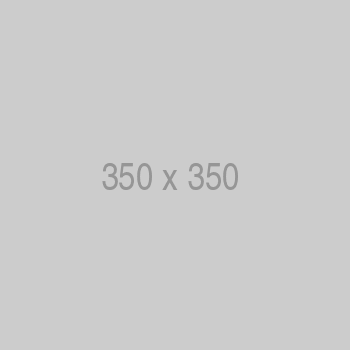
\includegraphics[width=\linewidth]{images/placeholder.png}
    (A)
  \end{minipage}
  \begin{minipage}{0.4\textwidth}
    \centering
    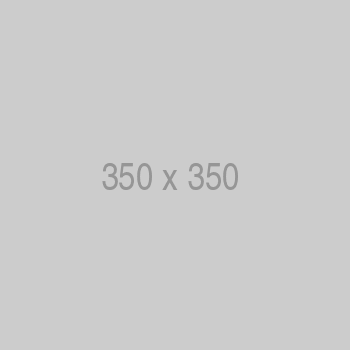
\includegraphics[width=\linewidth]{images/placeholder.png}
    (B)
  \end{minipage}
  \caption{Exemple de distortion introduite par une lentille à grand angle. (A) l'image originale (B) l'image rectifiée}
  \label{fig:distortion}
\end{figure}

Plusieurs modèles de distortion ont été proposés à travers le temps mais le plus répandu est celui radial-tangentiel, radial puisqu'il dépend de la distance du pixel par rapport au centre optique et tangentiel pour le déplacement des rayons tangentiel au cercle autour du centre optique. La distortion radiale-tangentielle peut-être exprimé par un polynôme permettant de mettre en correspondance les pixels de l'image originale $(x_c, y_c)$ en coordonnées normalisées aux pixels de l'image rectifiée $(u, v)$.

\begin{equation}
\begin{aligned}
  \hat{x}_c &= x_c\left(\frac{1 + \kappa_1r_c^2 + \kappa_2r_c^4 + \kappa_3r_c^6}{1 + \kappa_4r_c^2 + \kappa_5r_c^4 + \kappa_6r_c^6}\right) + 2p_1 x_c y_c + p_2(r_c^2 + 2 x_c^2) \\
  \hat{y}_c &= y_c\left(\frac{1 + \kappa_1r_c^2 + \kappa_2r_c^4 + \kappa_3r_c^6}{1 + \kappa_4r_c^2 + \kappa_5r_c^4 + \kappa_6r_c^6}\right) + p_1 (r_c^2 + 2 y_c^2) + 2p_2 x_c y_c \\
  r_c^2     &= x_c^2 + y_c^2
  \label{eq:rectification}
\end{aligned}
\end{equation}
\begin{equation}
\begin{aligned}
  u & = f_x \hat{x}_c + c_x\\
  v &= f_y \hat{y}_c + c_y
  \label{eq:focal_scaling}
\end{aligned}
\end{equation}
Les paramètres $\kappa_{[1-6]}$ sont les coefficients de distortion radial et $p_{[1,2]}$ les coefficients de distortion tangentiel. L'équation \ref{eq:focal_scaling} permet de mettre à l'échelle les coordonnées normalisées en coordonnées en pixels. Les paramètres de distortion et intrinsèques peuvent être estimés conjointement suivant la résolution d'un problème des moindres carrés non-linéaire \citep{Zhang2000}.

Bien que le modèle radial-tangentiel soit le plus populaire, entres-autres par sa présence dans la librairie de traitement d'images OpenCV, plusieurs auteurs proposent de nouveaux modèles avec divers avantages. Par exemple le modèle de distortion équidistant proposé par \citep{Kannala2006} est apte à modéliser la distortion à la fois de lentilles normales et de lentilles ultra-grand angle et le modèle par fonction rationelle de \citep{Claus2005} adapté aux lentilles grand-angle et catadioptriques. 

\subsection{Vision stereo}
\color{red}
Ajouter la théorie sur la géométrie épipolaire pour la résolution de profondeur par caméra stereo.
\color{black}

\subsection{Détection de lignes}

\begin{enumerate}
  \item canny
  \item HED
  \item Transformée de hough
  \item edlines
  \item lsd
\end{enumerate}
